% Chapters
\chapter{Sprint Planning}\label{chap:s4_sprintplanning}

\begin{chapterorganization}
  \item in \sectionref{sec:S4_bd} we describe the user stories we commit ourselves to during the \bd sprint planning meeting.
  \item in \sectionref{sec:S4_group} we describe the sprint planning in our group and lists our tasks with reference to a user story.
\end{chapterorganization}

\section{\bdtitle Sprint Planning}\label{sec:S4_bd}
During the \bd sprint planning we choose to work on the following user stories in this sprint. They are labeled with a number in parentheses for reference.

\todo{Tilføj conditions of satisfaction}

\begin{description}
  \item[Job Prioritization on Jenkins (1)] Developers have specified a desire for some jobs to have a higher priority than other jobs. For example developers would like libraries to run before apps.
  \item[Monkey Test on Debug Versions of Apps (2)] With the \db groups working on implementing database sync, they are making a test database available. Monkey tests currently use a development database that might be wiped accidentally. To ensure this does not happen monkey tests should run on debug APKs rather than release APKs.
  \item[Decrease Build Times on Jenkins Further (3)] When the queue on Jenkins is long, jobs can take a very long time to build. As we discussed in \sectionref{sec:non-emulator_testing}, the build times can be further reduces by working on the emulator.
  \item[Easy Download and Installation of all Apps (4)] In the previous sprint developers were not always using the latest versions of all apps, which lead to issues at the sprint end. The developers therefore want an easy way to download and install the newest version of all apps on their devices.
  \item[Document Jenkins Structure for Next Semester (5)] To make it easy for the next semester to start working with Jenkins, documentation of the Jenkins structure used is needed.
\end{description}

\section{Group Sprint Planning}\label{sec:S4_group}
At our internal sprint planning we divide the chosen user stories into tasks and estimate them. For this sprint, we have a total of 70 half days of work. \tableref{tab:sprint4_tasks} shows the tasks we have committed to solve for this sprint. Tasks with a plus (+) are tasks that have been added during the sprint as they were discovered.

\begin{table}%
  \centering
  \begin{tabular}{p{0.6\textwidth}rr}
    \toprule
    \textbf{Task} & \textbf{User Story} & \textbf{Estimation} \\
    \midrule
    Investigate conditions of satisfaction for our user stories & na & 2 \\
    Make a program to download and install the newest version of each app & 4 & 2 \\
    Make it so that the Android emulator is only started when no other devices are connected & 3 & 6 \\
    Connect to all Android devices wirelessly & 3 & 2 \\
    Connect Android devices permanently to the Internet & 3 & 2 \\
    Put debug APKs onto the ftp & 2 & 1 \\
    Make monkey tests use debug APKs & 2 & 1 \\
    Install Jenkins Prioritization Plugin & 1 & 1 \\
    Choose schedule for prioritization plugin & 1 & 2 \\
    Identify areas for Jenkins documentation (spike) & 5 & 2 \\
    Write about Jenkins files on server (from spike) & 5 & 2 \\
    Write about Jenkins structure (from spike) & 5 & 2 \\
    Investigate method to decrease emulator usage time (spike) & 3 & 1 \\
    % \midrule
    % \textbf{Down-prioritized tasks} & & \\
    % \midrule
    % \midrule
    % \textbf{Missed tasks} & & \\
    % \midrule
    % \textbf{Rejected tasks} & & \\
    % \midrule
    \midrule
    \textbf{Original total} & & y \\
    \textbf{Total} & & x \\
    \bottomrule
  \end{tabular}
\caption[Sprint 4 backlog]{Sprint backlog for sprint 4, excluding report tasks. The tasks are listed in no particular order.}
\label{tab:sprint4_tasks}
\end{table}

\todo{Tasken ``Investigate method to decrease emulator usage time (spike)''har vi ikke, men lavede uformelt den første dag da vi lavede sprint planning i gruppen}

\todo{I dette sprint skal vi også skrive frontmatter, backmatter, introduktion og konklusion}
\chapter{Improving Automated Testing}
\dummy

\section{Monkey Testing}
\dummy

\section{App Installation Test Case}
\dummy

\section{Code Coverage Reports}
We have a user story which states that Jenkins should provide code coverage metrics on for every project. This user story was generated by a group which were writing test of a database project, and wanted a measure of their progress. Their main request is for a percentage of LoC covered. A tool for code coverage report must at least provide this metric, but other more detailed metrics would also be nice to have. In version 0.10 of the New Android SDK Build System \parencite{new-build-android} support for the JaCoCo \parencite{jacoco-home} Java Code Coverage Library was included. It meets all of our demands for metrics, and is nicely integrated into the Android and Gradle build system. 
To make JaCoCo generate a report all one needs to do is to add the code shown in \listingref{lst:Jacoco} to the \mono{build.gralde} file of the project. 
\begin{gradlecode}[caption=Gradle script for enabling JaCoCo,label=lst:Jacoco]
dependencies {
    mavenCentral()
}
android {
    buildTypes {
        debug {
            testCoverageEnabled true
        }
    }
}
\end{gradlecode}{}
Now we generate code coverage reports locally and on Jenkins. We would like to also publish the code coverage results on Jenkins. There exists a Jenkins plugin for this purpose \parencite{jacoco-jenkins-plugin}. This plugin is easy to setup and provides detailed coverage statistics, and a overview with a percentage LoC covered. We use this plugin for publishing the code coverage metrics on Jenkins.
%!TEX root = ../report.tex
\section{Upload of Apps to Google Play}\label{sec:upload_google_play}
Jenkins compiles and builds the Giraf projects but does nothing with the generated APKs. One of the user stories selected in this sprint is \us{automatic upload of alpha releases to Google Play}.

Before the APKs can be published to Google Play, they need to be signed with a signature. The Android plugin for Gradle has functionality for automatic signing of APKs, and we will use this to sign. A keystore file is used to sign, and we are not interested in everybody having this file as it serves as a proof of identification. We save the file on the server, which means that it becomes impossible to build release versions of the apps locally using the Giraf keystore. When uploading a new app to Google Play, the version code of the new app must be greater than the version code of the app already in the app store. Incrementing the version code is not done per default, so we need to set up the build to increase the version code every time an app is successfully built. 

We have written a Gradle plugin handling this with the major part of this seen in \listingref{lst:gradle_versioncode}. The plugin keeps a properties file with the current version code for all apps. Upon executing the \mono{increaseVersionCode} Gradle task, it reads the version code (line 8) from the properties file and increments it (line 12). Then it writes it to the app manifest file (line 13), such that the build following will use the new version code. Finally, it updates the property file with the new version code (line 15), such that the next build will use this version code. If no current version code is found in the properties file (line 21), we assume the app is new and starts at version code \mono{1}, and as such we do not increment it (line 10).
\begin{gradlecode}[caption=Part of our Gradle plugin for updating version code,label=lst:gradle_versioncode]
project.task('increaseVersionCode') << {
    // [...]
    // Check to see if properties file exists.
    if (project.file(versionCodesFilePath).exists() != true) {
        throw new GradleException("No version code file found. Only Jenkins should run this task")
    }
    // [...]
    def newVersion = getVersionCode(project, applicationId)
    def versionCode = newVersion['value']
    if (!newVersion['created']) {
        // Increment version code if not new
        versionCode++
        // Write incremented version code to manifest
        // [...]
        // Write incremented version code back to properties file
        // [...]
    }
}

def getVersionCode(project, applicationId) {
    // Reads the version code from the properties file. Returns 1 if the version code does not exist.
}
\end{gradlecode}
 
Now that the APKs have been signed, they need to be uploaded to Google Play. This can be done in two ways: Via a Jenkins plugin \parencite{jenkins-play-plugin} or through Gradle \parencite{gradle-play-plugin}. The Jenkins plugin is easy to use, but requires that the exact name and location of the of the APK to upload is known. The Gradle plugin knows this already, since the information is already present in the Gradle build environment. Therefore we use Gradle to publish to Google Play via a Google Play API\@. After the APKs have been uploaded, they are moved to the ftp server which is hosted on the same machine as Jenkins in the directory \mono{/srv/ftp/}. This way the APKs are also available outside of the Google Play store.

\chapter{Restructuring of Jenkins}
The setup of Jenkins used in sprint 1 was tedious to work with since all jobs were configured independently. If a change had to be made to several jobs, we would have to manually configure the change in each job. Not only did this take a considerable amount of time, but it was also prone to human errors during the process. In this sprint, we have to make small modifications to all jobs several times. This would be very tedious, so we have decided make job configurations easier to manage, even though it is not connect directly to a story. We consider it refactoring.
 The jobs on Jenkins are generally very similar in their configuration. We can benefit from having a base configuration, which the jobs only modify. There exists a Jenkins plug-in for this, called inheritance-plugin\parencite{jenkins-inheritance}. With this plug-in installed, whenever we decide to make a change to e.g.\ the build system, it will not be necessary to change this in each job. Instead, the change can be made on the base job, and all relevant jobs will inherit this change. This also ensures that jobs follow a consistent pipeline and thus do not differ in from job to job.

The plug-in requires the jobs to be of a special \emph{inheritable} type. We therefore have to covert the existing jobs to inheritable jobs to take advantage of this. As it is impossible to convert a existing job to the inheritable type, we have to re-create all the jobs again. This is not that big of a deal, as the time to setup will be considerably shorter when taking advantage of the inheritable job type. When the old jobs are removed the build history will be lost. This is a minor nuisance but we consider it a small price to pay, compared to the advantages. When deciding how to structure the build, we see two general categories that are sufficiently distinct: Android apps and Android libraries. We create an abstract job for each of these. They do overlap somewhat in functionality, which means we have to create an abstract job for each job task. As such we create abstract jobs for e.g.\ \emph{run Gradle}, \emph{run unit tests}, \emph{find and move APKs}, and \emph{publish lint report}. The abstract jobs \emph{Android app} and \emph{Android library} inherit from the small abstract tasks that are relevant.

We have modelled this as an OOP class diagram in \todo{Pæn graf over Jenkins jobs og inheritance? JA!}


\chapter{Improving Build Times}
The project groups want the build times on Jenkins to be faster. When multiple changes are pushed to the master branch within a short space of time, they will create congestion the build queue. This means that even though the build itself may take only a few minutes, the time it takes from push to finished build may be much longer.

To identify in which parts of the build process to make faster, we measure the time different parts of the Launcher project take. The Launcher project is the main application which depends on many other subprojects. The timings are measured on the Jenkins server and shown in \figureref{fig:launcher_build_times_1}. The shows the build timings of the Launcher application and the different subprojects (\emph{Oasis-lib, Giraf-Component, Local-db, Barcode-scanner, and Metadata}), as well as the startup time for the emulator. As can be seen, the emulator and the Giraf-component and Oasis-lib projects have the most significant influence on build times. These three parts use about \SI{90}{\percent} of the total build time.

To understand which parts of the subprojects that take time, we measure the individual build steps (tasks) performed during a build. These can be seen in \appendixref{app:build_times}. The reason that the Oasis-lib subproject takes a long time to build is that it contains a great number of tests which run on the emulator. These tests are run every time a project depending on Oasis-lib builds --- even though the library itself has not been updated. The most significant task when building the Giraf-Component library is the test task as well. However, the Giraf-Component library only contains one simple test, so we do not expect the actual test execution time to use much of this time. Instead, we expect it to be caused by the order in which projects are tested. When preparing the tests, the tests from all projects are combined into a single Android application package (APK-file). The first test task run is responsible for installing this application on the emulator, while the subsequent test tasks can skip this step. Because the Giraf-components project is the first in the sequence of libraries to be tested, this task also installs the tests on the emulator which is likely to take some time.
\todo{Overvej flere målinger og tag gennemsnit}
\begin{figure}
  \centering
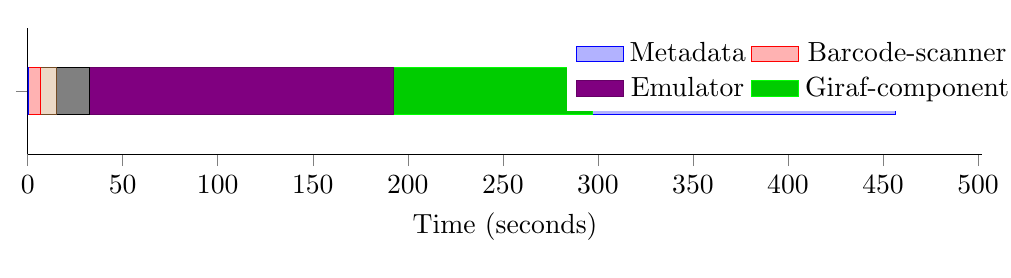
\begin{tikzpicture}[trim axis left, trim axis right]
  \begin{axis}[
    xbar stacked,
    scale only axis,
    width=\textwidth,
    axis y line*= none, axis x line*= bottom,
    %xmajorgrids = true,
    ytick = data,
    yticklabels = {},
    tick align = outside,
    %xtick pos = left,
    bar width=6mm,
    y=8mm,
    %nodes near coords,
    legend style={
      legend columns=4,
      anchor=north,
      yshift=0ex,
      xshift=0ex,
      draw=none
      %legend cell align=left
    },
    area legend,
    xlabel = {Time (seconds)},
    xmin = 0
  ]
    \addplot coordinates
    {(0.2,0)};
    \addlegendentry{Metadata}
    \addplot coordinates
    {(6.625,0)};
    \addlegendentry{Barcode-scanner}
    \addplot coordinates
    {(8.393,0)};
    \addlegendentry{Launcher}
    \addplot coordinates
    {(17.223,0)};
    \addlegendentry{Local-db}
    \addplot coordinates
    {(160.000,0)};
    \addlegendentry{Emulator}
    \addplot coordinates
    {(104.696,0)};
    \addlegendentry{Giraf-component}
    \addplot coordinates
    {(159.497,0)};
    \addlegendentry{Oasis-lib}
    %\legend{Test, test, test, test, test, test}
  \end{axis}
\end{tikzpicture}
\caption{Timings during build of the Launcher project before updating emulator plugin.}\label{fig:launcher_build_times_1}
\end{figure}

To improve the overall build times, we look at how to speed up the emulator and to avoid running tests on the dependencies every time a project is build. We first update the Android Emulator Jenkins plugin to a new version with improved emulator stability. We do this to ensure that we do not work on improving parts which are already improved in the most recent version of the plugin. After updating, we measure the build times again. As shown in \figureref{fig:launcher_build_times_2}, the emulator startup time is significantly increased. Because of this, the emulator startup time is no longer a concern, and we focus solely on decreasing the subproject build times.
\begin{figure}
\centering
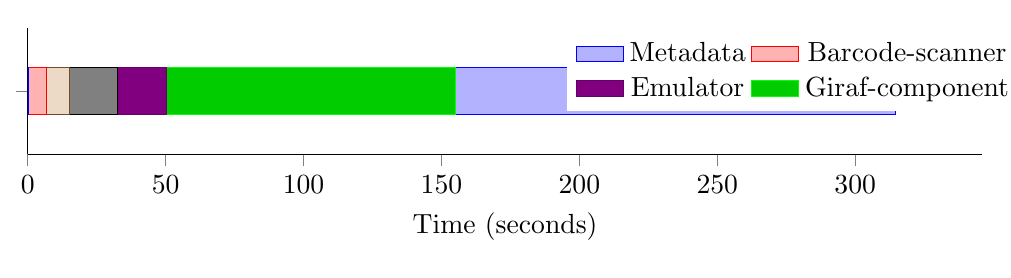
\begin{tikzpicture}[trim axis left, trim axis right]
  \begin{axis}[
    xbar stacked,
    scale only axis,
    width=\textwidth,
    axis y line*= none, axis x line*= bottom,
    %xmajorgrids = true,
    ytick = data,
    yticklabels = {},
    tick align = outside,
    %xtick pos = left,
    bar width=6mm,
    y=8mm,
    %nodes near coords,
    legend style={
      legend columns=4,
      anchor=north,
      yshift=0ex,
      xshift=0ex,
      draw=none
      %legend cell align=left
    },
    area legend,
    xlabel = {Time (seconds)},
    xmin = 0
  ]
    \addplot coordinates
    {(0.209,0)};
    \addlegendentry{Metadata}
    \addplot coordinates
    {(6.625,0)};
    \addlegendentry{Barcode-scanner}
    \addplot coordinates
    {(8.393,0)};
    \addlegendentry{Launcher}
    \addplot coordinates
    {(17.223,0)};
    \addlegendentry{Local-db}
    \addplot coordinates
    {(18.000,0)};
    \addlegendentry{Emulator}
    \addplot coordinates
    {(104.696,0)};
    \addlegendentry{Giraf-component}
    \addplot coordinates
    {(159.497,0)};
    \addlegendentry{Oasis-lib}
    %\legend{Test, test, test, test, test, test}
  \end{axis}
\end{tikzpicture}
\caption{Timings during build of the Launcher project.}\label{fig:launcher_build_times_2}
\end{figure}



% TODO: Undgå at teste dependencies: Vi har brug for at styre vores binære filer
\chapter{Sprint Review}\label{chap:sprint3_end}

\begin{chapterorganization}
  \item in \sectionref{sec:s2_goals} we evaluate how the sprint went and whether we reached our goals on a group level.
  \item in \sectionref{sec:s2_multiprj_review} we evaluate how the sprint went on the multi project level.
\end{chapterorganization}

\section{Sprint Goals}\label{sec:s3_goals}
\dummy

\section{Multi-Project Sprint Review}\label{sec:s3_multiprj_review}
\dummy
